Fysikeren Michael Faraday beskrev, hvordan et skiftende magnetisk flux er i stand til at danne en elektrisk strøm. Den magnetiske flux angiver størrelsen på magnetfeltet i forhold til det givne areal, magnetfeltet påvirker. Den magnetiske flux afhænger af forskellige parametre, som spiller ind på at danne den elektriske strøm.

Den magnetiske flux er styret af arealet, den påvirker. Hvis størrelsen på det givne areal ændres, vil der også ske en ændring i den magnetiske flux. Hvis det gældende areal mindskes, vil den elektriske flux mindskes. Modsat vil en forøgelse af arealet medvirke, at den magnetiske flux øges.

\begin{figure}[H]
\includegraphics[scale=0,5]{Vildledning/Schematics/Areal_vs_Bfelt}
\end{figure}

Størrelsen på arealet, der bliver påvirket, er ikke kun afgjort af arealets dimentionen, men også vinklen for, hvordan den magnetiske feltlinjer står ind på det givne areal. Hvis feltlinjerne står vinkelret på det gældende areal, vil flest mulige feltlinjer rammen arealet. Hvis arealet står vinklet under 90 grader, vil nogle af feltlinjerne ikke løbe igennem og påvirke arealet, og den magnetiske flux mindskes. Er arealet parallelt med de magnetiske feltlinjer, så vil så få magnetiske feltlinjer som muligt påvirke arealet. Når vinklen ændres for de magnetiske feltlinjer og arealet, så vil den magnetiske flux også ændres.

\begin{figure}[H]
	\centering
	\begin{minipage}[b]{0.48\textwidth}
	\centering
	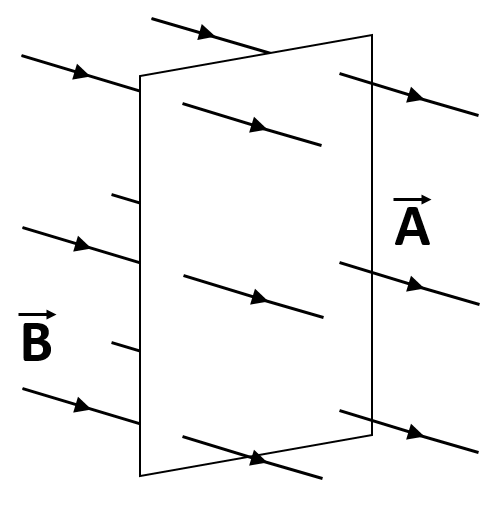
\includegraphics[width=0.5\textwidth]{Vildledning/Schematics/Magnetfelt_vinkelret} % Venstre billede
	\end{minipage}
	\hfill
	\begin{minipage}[b]{0.48\textwidth}
	\centering
	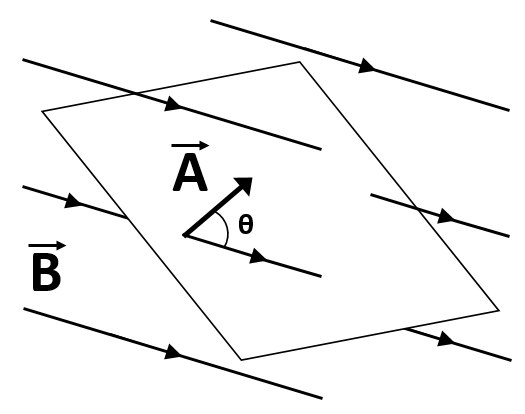
\includegraphics[width=0.5\textwidth]{Vildledning/Schematics/Magnetfelt_vinklet} % Højre billede
	\end{minipage}
\end{figure}

Størrelsen for de magnetiske feltlinjer er påvirket af strømstyrken for systemet. Ved en ændring af strømstyrken, vil de magnetiske feltlinjer ændre størrelse, hvorved den magnetiske flux vil varriere.